\documentclass[border=3pt,tikz]{standalone}
% Shared look for every TikZ figure in these notes.
% Included by each standalone figure file; also keeps the figures consistent
% with the colours used in the PDF and on the website.

\usepackage{tikz}
\usepackage{pgfplots}
\pgfplotsset{compat=1.18}
\usetikzlibrary{arrows.meta, decorations.markings, decorations.pathmorphing,
                patterns, calc, positioning}
\usepackage{amsmath}

% Series colours are the three validated categorical slots also used by the
% interactive widgets, so a path drawn in the printed notes and the same path on
% the website are the same colour. They clear the colour-vision-deficiency and
% contrast checks as a set; every path is direct-labelled as well, so colour is
% never the only thing carrying identity.
\definecolor{duPurple}{HTML}{68246D}
\definecolor{duBlue}{HTML}{2A78D6}
\definecolor{duRed}{HTML}{EB6834}
\definecolor{duGreen}{HTML}{1BAF7A}
\definecolor{duGrey}{HTML}{6B6B6B}

\tikzset{
  axisline/.style   = {-{Stealth[length=3mm]}, line width=0.7pt, black},
  path1/.style      = {duBlue,   line width=1.1pt},
  path2/.style      = {duRed,    line width=1.1pt},
  path3/.style      = {duGreen,  line width=1.1pt},
  statedot/.style   = {circle, fill=black, inner sep=1.4pt},
  arrowhead/.style  = {decoration={markings,
                        mark=at position #1 with {\arrow{Stealth[length=2.6mm]}}},
                       postaction={decorate}},
  lbl/.style        = {font=\small},
  slbl/.style       = {font=\footnotesize, duGrey},
  workfill/.style   = {duPurple, opacity=0.16},
}

% Corollary 8: any process a from 1 to 2, closed by a reversible process b
\begin{document}
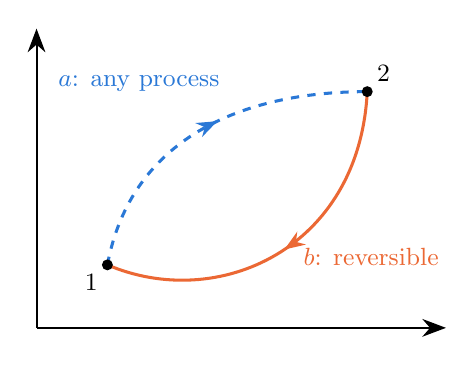
\begin{tikzpicture}[x=1cm,y=1cm]
  \draw[axisline] (0,0) -- (5.2,0);
  \draw[axisline] (0,0) -- (0,3.8);
  \coordinate (A) at (0.9,0.8); \coordinate (B) at (4.2,3.0);
  \draw[path1, dashed, arrowhead=0.55] (A) .. controls (1.2,2.4) and (2.6,3.0) .. (B);
  \draw[path2, arrowhead=0.5] (B) .. controls (4.1,1.0) and (2.3,0.2) .. (A);
  \node[statedot] at (A) {}; \node[lbl, below left] at (A) {1};
  \node[statedot] at (B) {}; \node[lbl, above right] at (B) {2};
  \node[lbl, duBlue, align=center] at (1.3,3.1) {$a$: any process};
  \node[lbl, duRed] at (4.25,0.9) {$b$: reversible};
\end{tikzpicture}
\end{document}
